\chapter{Implementation}

\textbf{Author: } 

\section{Generating test data}
Good test data is of utmost importance in machine learning. The system can only know information that is depicted in the training data, which is why it is important to include as many aspects of the problem as possible in this data.

Since machine learning needs a lot of data in order to solve the given task it can be tiresome to generate and label all this data by hand. Therefore the authors decided to simulate the objects and the camera using a computer graphics modelling software called Blender.

Blender allows for relatively easy generation of training data by providing a Python API.

[TODO: Image camera setup, lightning, objects in Blender]

[TODO: Renders and labels for example objects]

\section{OpenCV}
OpenCV is a framework for image manipulation. Some of its use cases are changing the colour spectrum, filtering the image by colour and cropping images. The authors use OpenCV to test whether there are differences between filters for the images in the training data, for example greyscale images compared to coloured images. An example render, which OpenCV gets as an input can be seen in Figure~\ref{pic:implementation_opencv_original}.

\begin{figure}[h!]
	\centering
	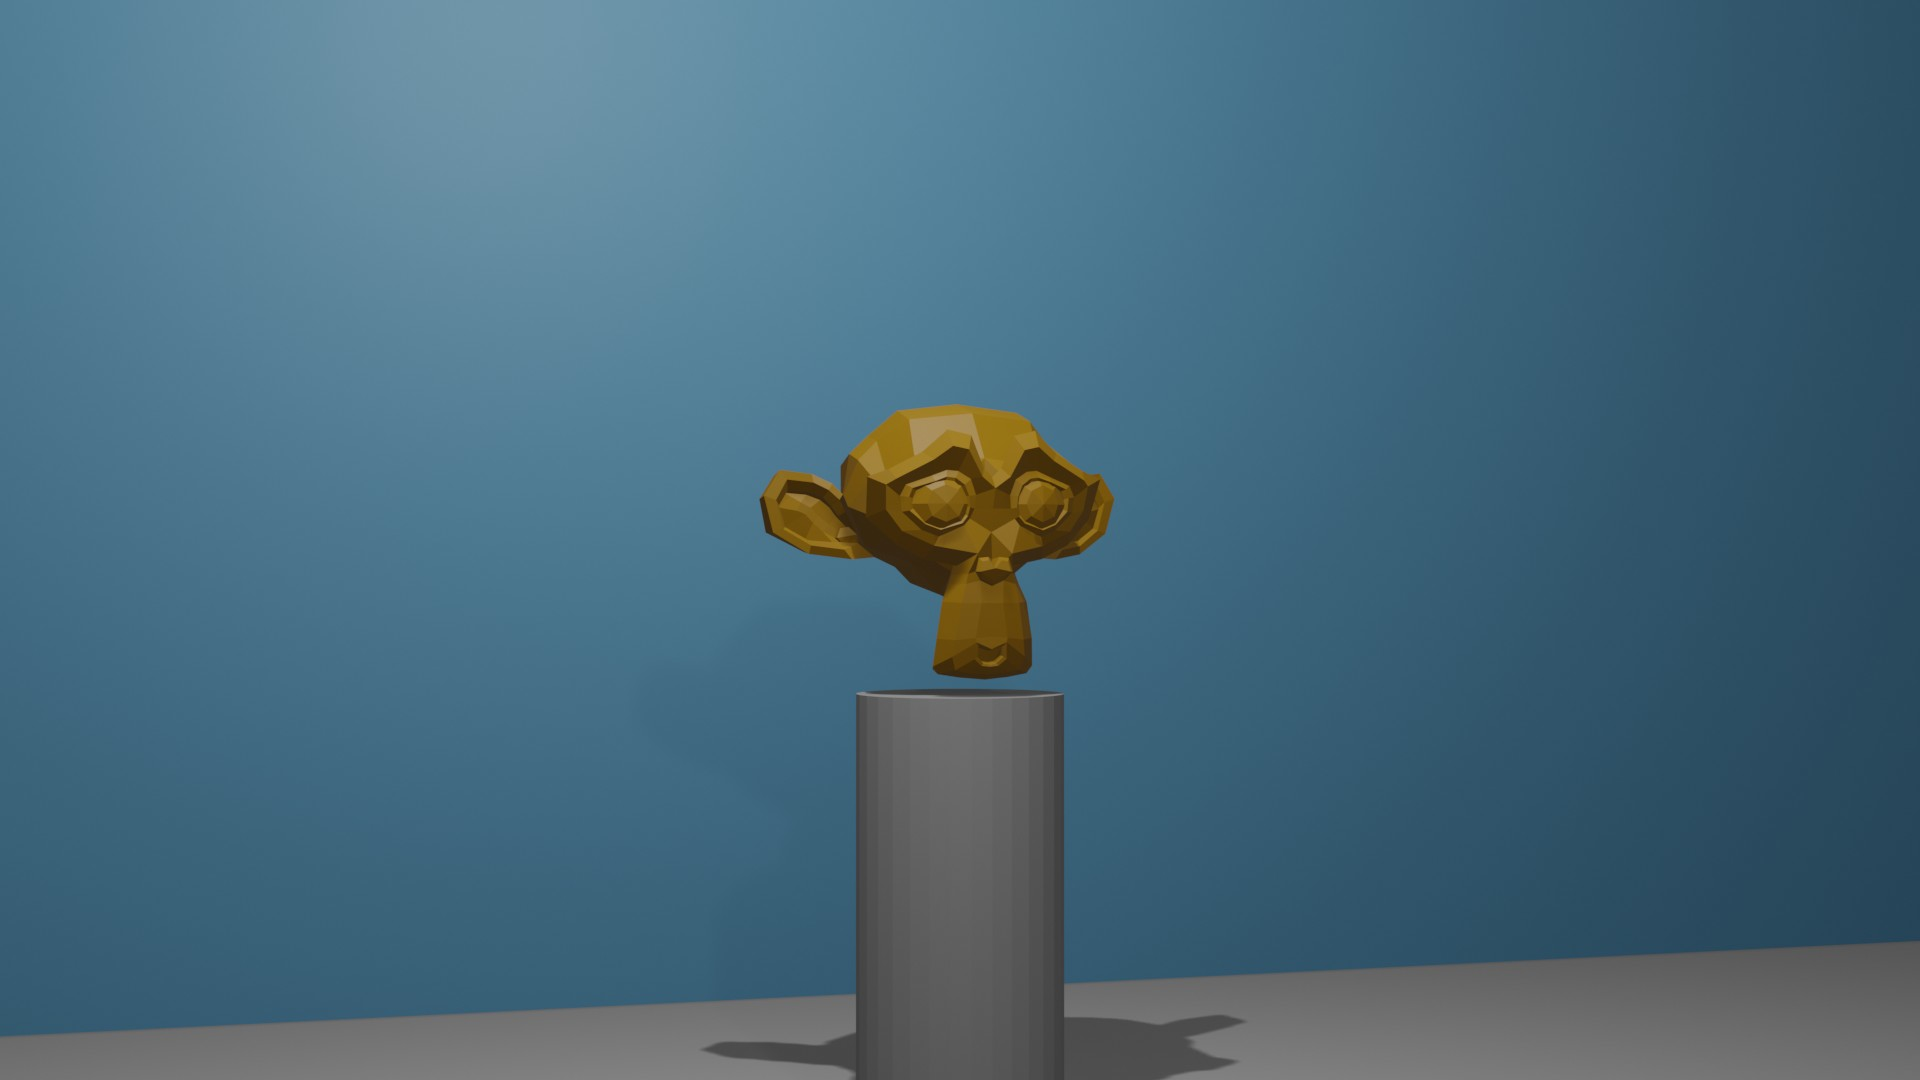
\includegraphics[width=5in]{img/implementation_opencv_original.png}
	\caption{One of two original renders produced by Blender, both depicting the same object from different points of view.}	%22_2
	\label{pic:implementation_opencv_original}
\end{figure}

\subsection{Greyscale}
Converting an image into greyscale can easily be achieved by the following OpenCV code:

[TODO: How is the image converted? (Average of all three channels?, ...)]

\begin{lstlisting}[language=python]
import cv2

image = cv2.imread('path/to/image')
image_greyscale = cv2.cvtColor(image, cv2.COLOR_BGR2GRAY)
cv2.imwrite('path/for/saving/greyscale/image', image_greyscale)
\end{lstlisting}

This code first reads the image into 'image'. Then it converts the color of 'image' into a greyscale format and stores the result into 'image\_greyscale', which is then written to the specified path. The output generated by this code is depicted in Figure~\ref{pic:implementation_opencv_greyscale}.

\begin{figure}[h!]
	\centering
	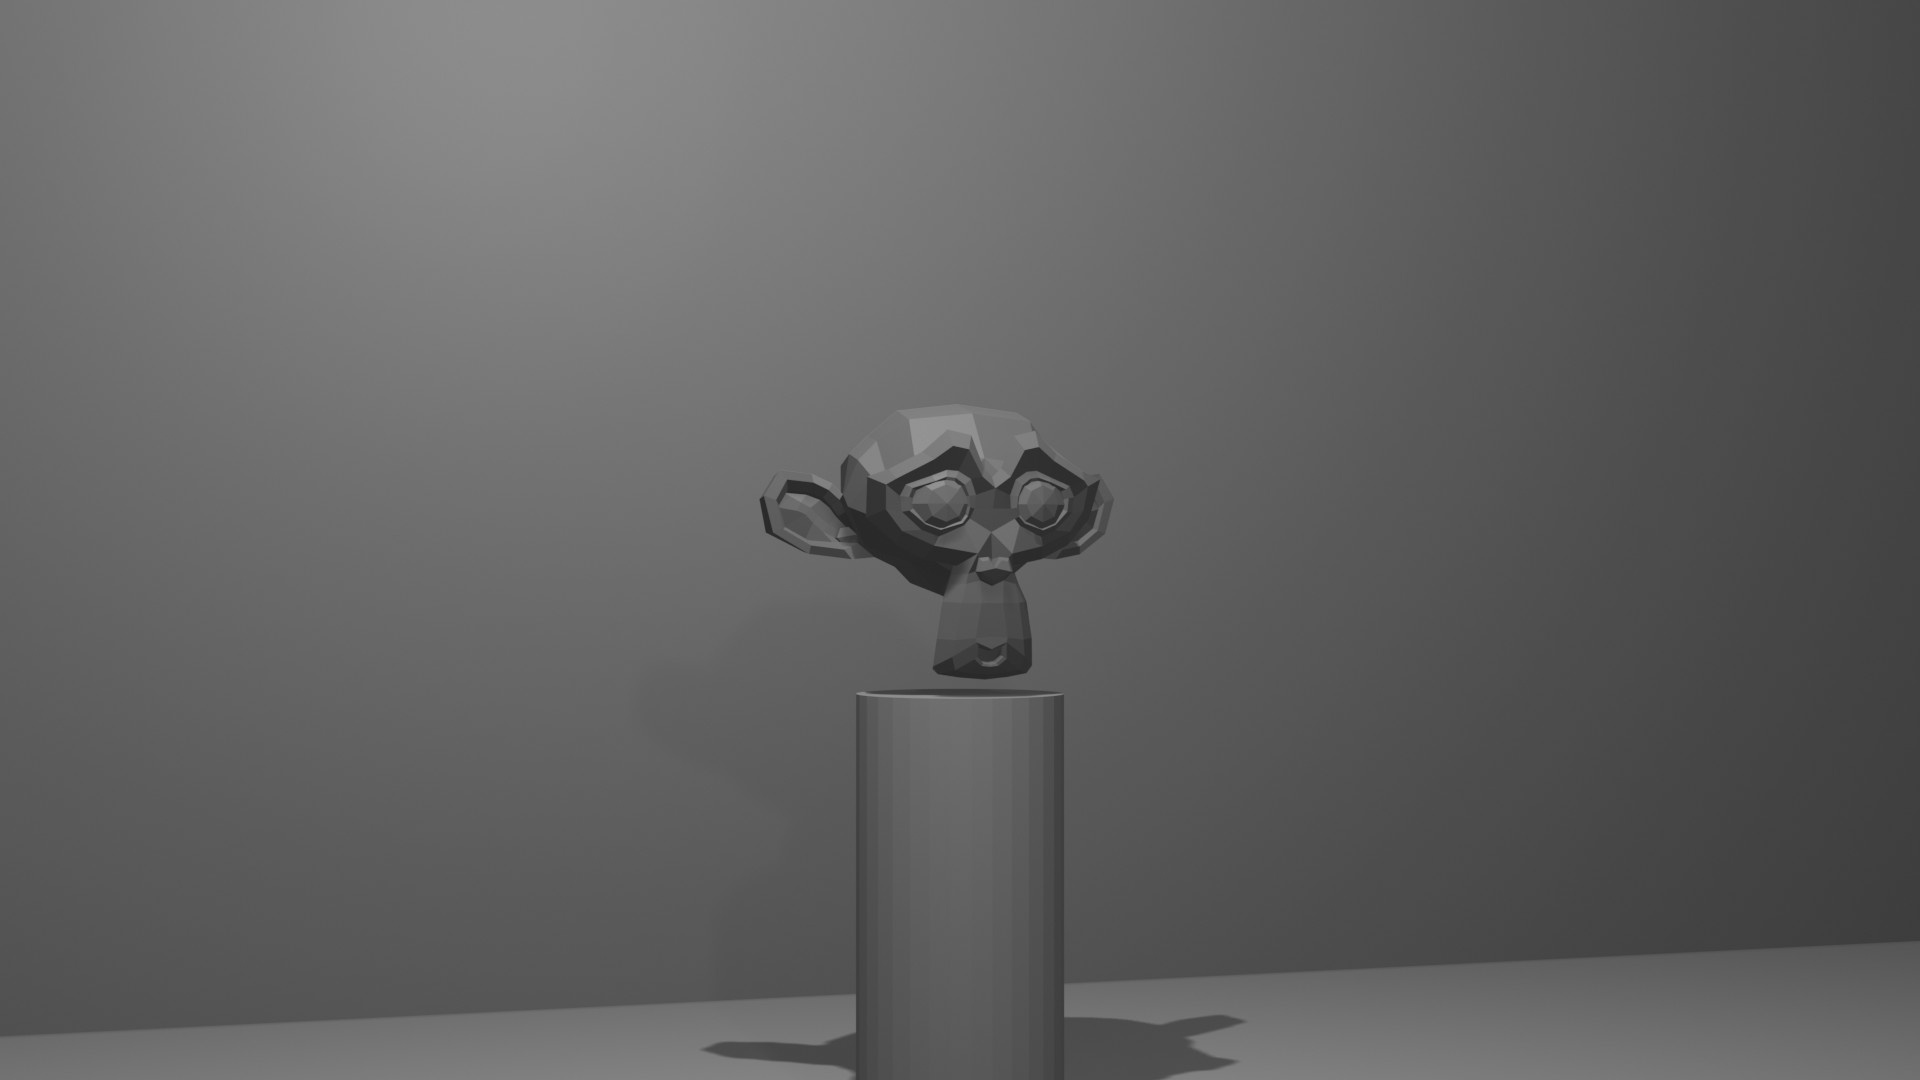
\includegraphics[width=5in]{img/implementation_opencv_greyscale.png}
	\caption{The greyscale image produced by OpenCV.}
	\label{pic:implementation_opencv_greyscale}
\end{figure}

The advantage of using greyscale images in Neural Networks is the simplification of the input layer. In greyscale images each pixel can be represented by a single decimal value between 0 and 1. This enables the first layer of the neural network to be two dimensional instead of the three dimensional counterpart, where each pixel is represented by the three decimal values for the red, green and blue colour channels.

\subsection{Resolution}
By reducing the resolution of an image the density of pixels is lessened. In this process information, that can not be regained, is lost. The OpenCV code for downscaling the images used by the authors is the following:

\begin{lstlisting}[language=python]
import cv2

image = cv2.imread('path/to/image')

scale_percent = 10  # percent of original size
width = int(image.shape[1] * scale_percent / 100)
height = int(image.shape[0] * scale_percent / 100)
dim = (width, height)

downscaled = cv2.resize(image, dim)
cv2.imwrite('{}/{}'.format(newdir_path, filename), downscaled)
\end{lstlisting}

OpenCV provides a resize function, which takes an image and the new dimensions of the image as an argument and outputs the resized image. To make sure the aspect ratio stays the same new image dimensions are calculated as a percentage of the original ones.

The output image of this code can be found in Figure~\ref{pic:implementation_opencv_resolution}.

\begin{figure}[h!]
	\centering
	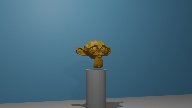
\includegraphics[width=4.5in]{img/implementation_opencv_resolution.jpg}
	\caption{Image with lower resolution than the original one. Due to the fact that the image is displayed in the same size as Figure~\ref{pic:implementation_opencv_original}, the pixel size in this image appears larger.}
	\label{pic:implementation_opencv_resolution}
\end{figure}

\subsection{Cropping}

Cropping an image can remove unnecessary or unwanted parts of an image by simply cutting off areas. This is often wanted in photography to only keep what is interesting in a photo and to shift the view of the viewer to specific areas. However, the author's guess that cropping an image will worsen performance of the neural network, because information of the relative sizes are partly lost. It basically compares to zooming into the image.

\begin{figure}[h!]
	\centering
	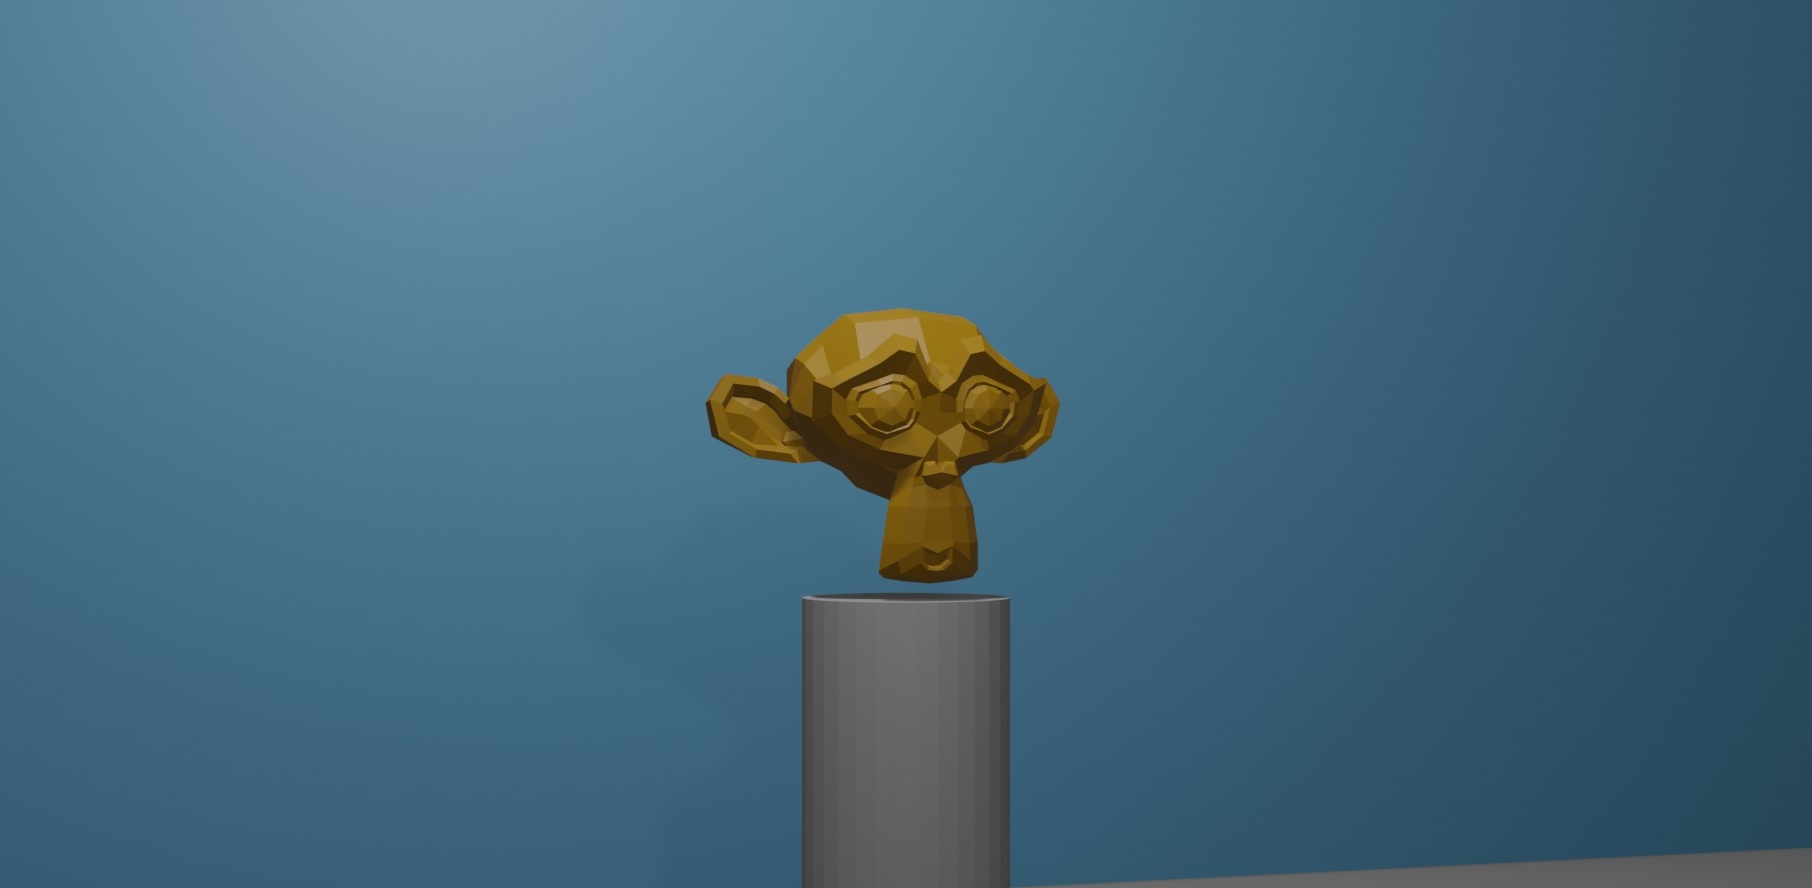
\includegraphics[width=4.5in]{img/implementation_opencv_cropping.jpg}
	\caption{Comparison between normal and a cropped image.}
	\label{pic:implementation_opencv_cropping}
\end{figure}

\subsection{Saturated}

A saturated image has greater strength of colours, basically making them more distinguishable from each other. If an image is not saturated enough, colours appear as "washed out" and differences in colour are difficult to determine. Therefore, in order to help the neural network, the authors decided to also test with saturated versions of these images.

\begin{figure}[h!]
	\centering
	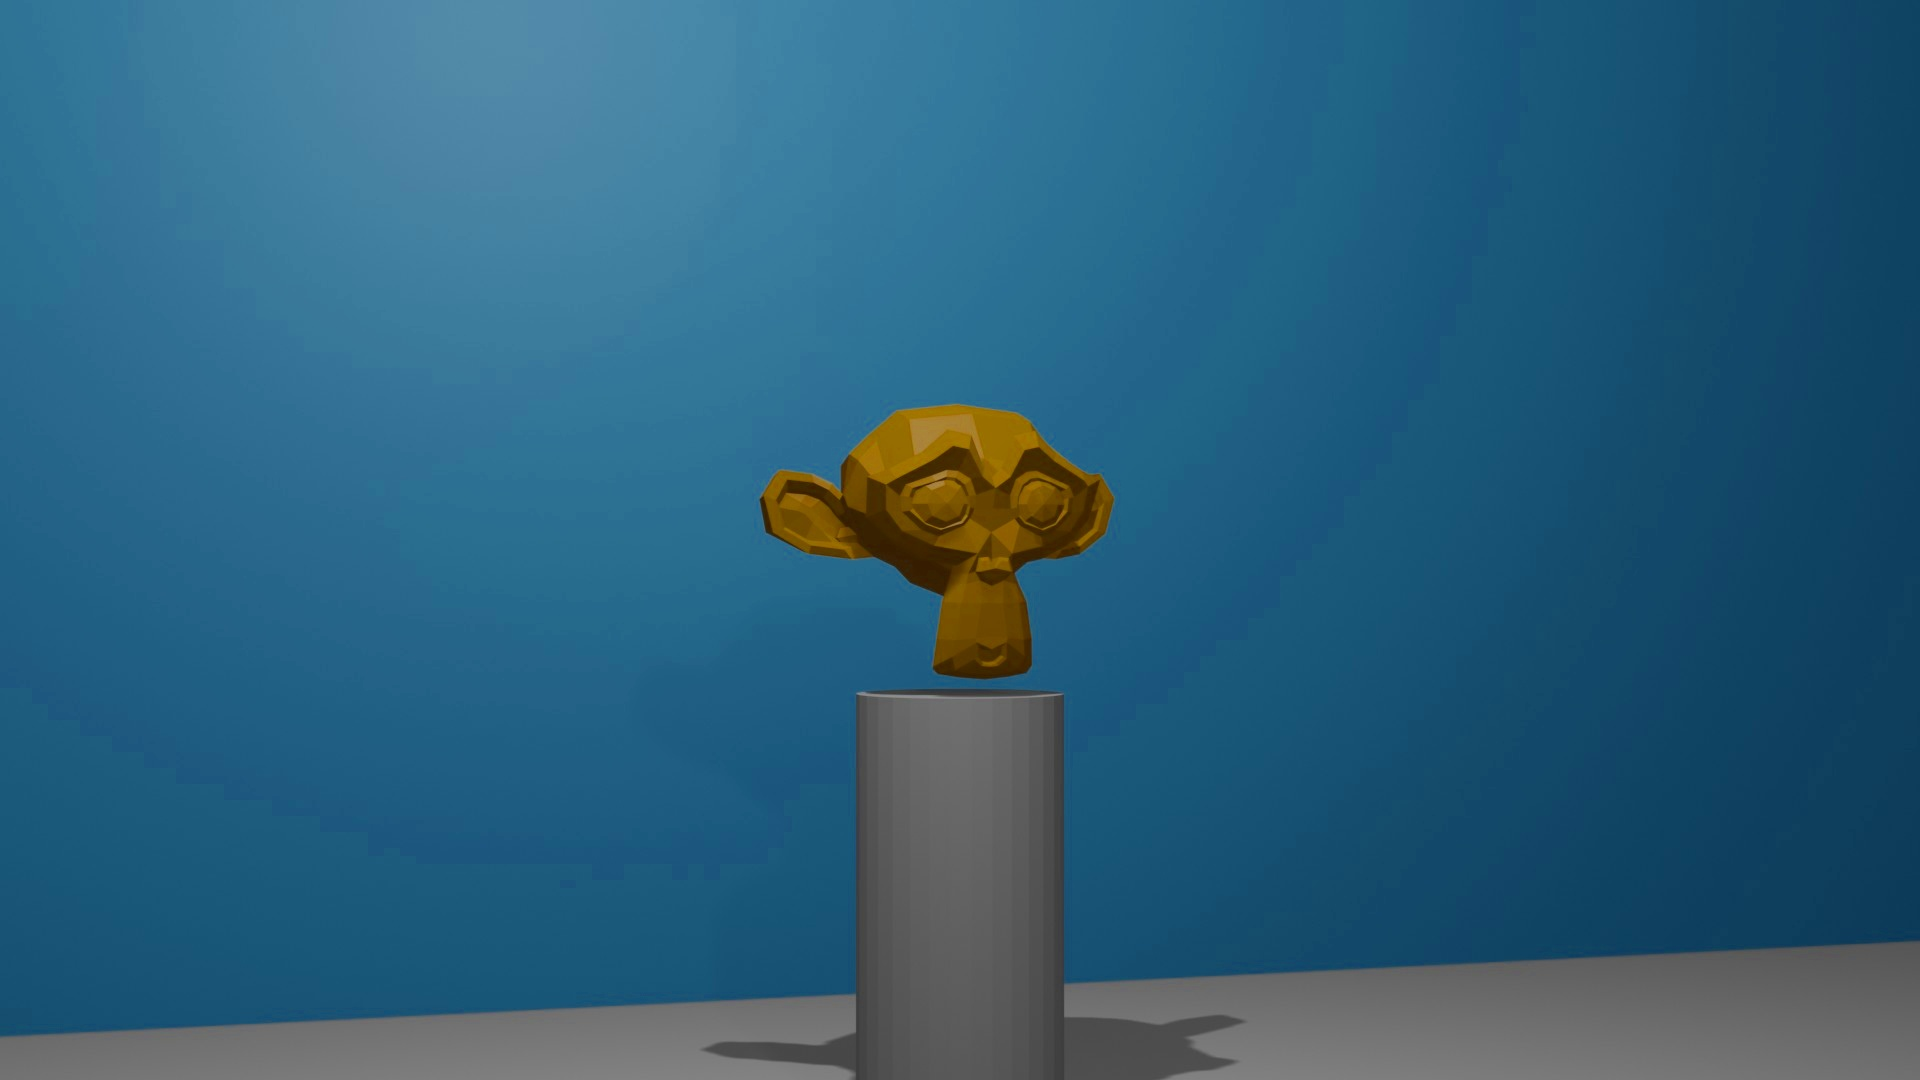
\includegraphics[width=4.5in]{img/implementation_opencv_saturated.jpg}
	\caption{Comparison between normal and saturated image.}
	\label{pic:implementation_opencv_saturated}
\end{figure}


\subsection{Brightness}

Because the neural network should also work in different environment, where other methods could have problems, the authors also tested with overly bright images. This makes it very hard to notice dark areas, such as shadows, to help with distances and scaling.

\begin{figure}[h!]
	\centering
	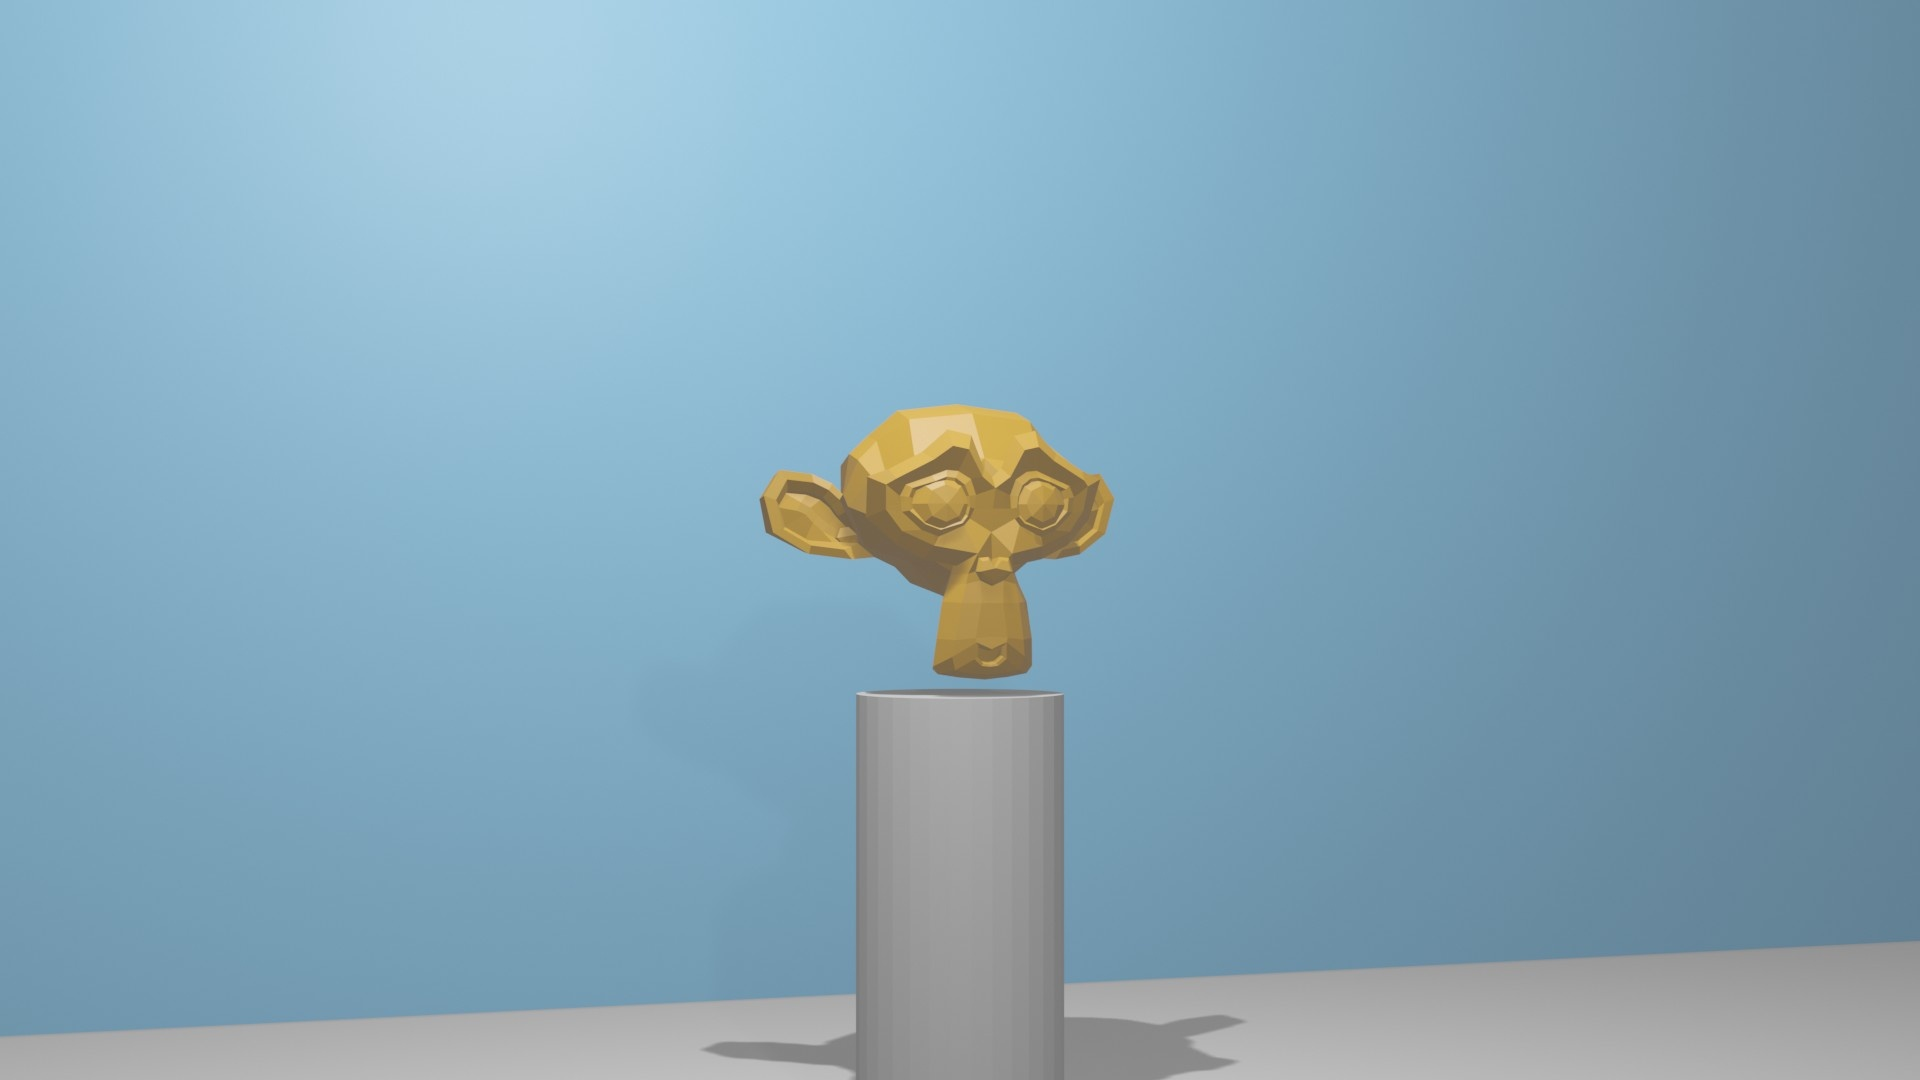
\includegraphics[width=4.5in]{img/implementation_opencv_brightness.jpg}
	\caption{Comparison between normal and brightness image.}
	\label{pic:implementation_opencv_brightness}
\end{figure}

\section{Neural Network}
\subsection{Structure of our Neural Network}

[wie lesen wir Daten ein, wie viele layer, was ist der output (maximale entfernung? z.B. 10m)]

\section{C++ Implementation}

\section{Technical difficulties}

\filbreak
